\section{Runtime System}\label{sec:runtime-system}
The runtime system of Parallel.es consists of two parts: Firstly, the slaves running in background threads executing the tasks and secondly, the public API in the main thread forming the facade and acting as the master for the slaves. Applications are using the facade provided by the master to run a function in a background thread. The master is responsible for spawning the slaves and distributing the work onto these. Hence, a thread pool is used to manage the created slave instances and queue the tasks if no idle slave is available. The default thread pool uses a FIFO queue, and the number of slaves is limited to the number of logical processors provided by the hardware\footnote{The number of logical processors can be determined using \javascriptinline/navigator.hardwareConcurrency/. The runtime system assumes that the hardware has four logical processors if the used browser does not support this API.}. The next section describes how the runtime system executes a single task. 

\subsection{Task Execution}
The steps needed to process a single task are shown in \cref{fig:runtime-system}. The application passes the task function together with the arguments for its invocation to the facade that acts as the master (1). The thread pool, residing in the master, selects an idle slave to execute the task or queues the task until a slave gets available. The master then transmits the structured cloned representation of the function call --- consisting of a unique id identifying the task function and the arguments for the task function invocation --- to this slave (2). The slave performs a lookup in the function cache to obtain the function with the given id (3). If the task function is executed for the first time on this slave instance, then it is not present in the function cache and, therefore, the slave requests the definition from the master (4). The master transmits the function definition to the slave (5) which deserializes and registers the function in the function cache (6). The slave calls the deserialized task function with the provided arguments (7) and returns the structured cloned result back to the master (8). The master invokes the success handler in the main thread to hand the result over to the application (9). 

\begin{figure*}
	\centering
	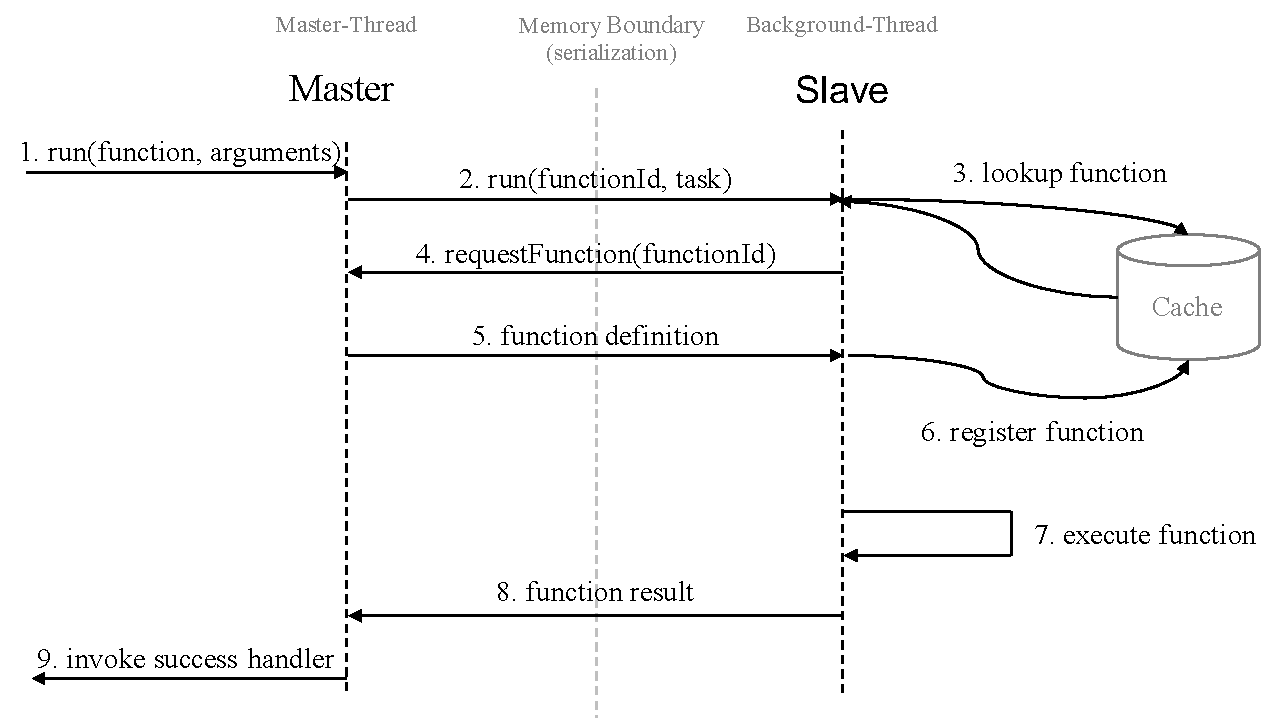
\includegraphics[width=0.8\textwidth]{runtime-system.pdf}

	\caption{Parallel.es Runtime System}
	\label{fig:runtime-system}
\end{figure*}

The caching of the function definitions on the slave has the advantage that performed JIT-optimizations are not thrown away if a task has completed. The caching can be especially useful for frequent but short running tasks for which the serialization and JIT-optimization overhead weight heavier.


\subsection{Limitations}
The current runtime system supports the essential features. However, it misses support for asynchronous task operations and runtime environments other than the browser. There are no conceptual or technical reasons for not supporting either of these features. 